\documentclass{beamer}
\usepackage[english]{babel}
\usepackage[utf8]{inputenc}
\usepackage[T1]{fontenc}
\usepackage{graphicx, tikz, multicol, wrapfig}
\usepackage[framemethod=TikZ]{mdframed}


\mode<presentation>
{
    \usetheme{Boadilla}
    \usecolortheme{default}
    \usefonttheme{default}
    \setbeamertemplate{navigation symbols}{}
    \setbeamertemplate{caption}[numbered]
} 


\title[H-SPACE, Budapest 2019]{Exploitation of Sentinel-1 SAR data for studying geodynamic, tropospheric and ionospheric processes.}
\author[Bozsó et al.]{István Bozsó, Eszter Szűcs, László Bányai, Viktor Wesztergom}
\institute[MTA CSFK GGI]{MTA CSFK Geodetic and Geophysical Institute}
\date{2019.02.28.}

\def\rar{\rightarrow}
\def\lar{\leftarrow}

\newcommand\quo[1]{``#1''}
\newcommand\subt[2]{#1_{\text{#2}}}
\newcommand\pard[2]{\frac{\partial #1}{\partial #2}}
\newcommand\abs[1]{\left|#1\right|}


\newcommand\inc[1] {
    \includegraphics[width=\textwidth]{#1}
}

\newcommand\img[2] {
    \includegraphics[width=#2\textwidth]{#1}
}

\newenvironment{ffig}[1]
{
    \begin{mdframed}[linecolor=#1, linewidth=5.0pt, roundcorner=5pt,
                     innerrightmargin=10pt, innerleftmargin=10pt,
                     innertopmargin=0pt, innerbottommargin=5pt,
                     skipabove=0pt, skipbelow=0pt,
                     backgroundcolor=white, frametitle={}, align=center]
    \begin{center}
}
{
    \end{center}
    \end{mdframed}
}

\newenvironment{fig}[1]
{
    \begin{minipage}{#1\textwidth}
    \begin{center}
}
{
    \end{center}
    \end{minipage}
}


\newcommand{\fcap}[1] {
    \captionof{figure}{#1}
}

\newcommand{\genenv}[1] {
    \def\b#1 { \begin{#1} }
    \def\e#1 { \end{#1} }
}


\def\bffig { \begin{ffig} }
\def\effig {   \end{ffig} }

\def\bfig { \begin{fig} }
\def\efig {   \end{fig} }

\def\bitz { \begin{itemize} }
\def\eitz {   \end{itemize} }

\def\bmini { \begin{minipage} }
\def\emini {   \end{minipage} }

\def\bcent { \begin{center} }
\def\ecent {   \end{center} }

\def\fcol{\color{blue!55!black}}

\newcommand{\fig}[1]{
    \begin{mdframed}[linecolor=blue!65!white, linewidth=1.75pt, roundcorner=0.75pt,
                     innerrightmargin=0pt, innerleftmargin=0pt,
                     innertopmargin=0pt, innerbottommargin=0pt,
                     backgroundcolor=white, frametitle={}, align=center]
        \includegraphics[width=1.0\textwidth]{#1}
    \end{mdframed}
}

\newcommand{\figm}[2]{
    \begin{center}
    \begin{minipage}[c]{#2\textwidth}
    \begin{mdframed}[linecolor=blue!65!white, linewidth=1.75pt, roundcorner=0.75pt,
                     innerrightmargin=0pt, innerleftmargin=0pt,
                     innertopmargin=0pt, innerbottommargin=0pt,
                     backgroundcolor=white, frametitle={}, align=center]
        \includegraphics[width=1.0\textwidth]{#1}
    \end{mdframed}
    \end{minipage}
    \end{center}
}

\newenvironment{minic}[1]
{
    \begin{center}
    \begin{minipage}[c]{#1\textwidth}
}
{
    \end{minipage}
    \end{center}
}


\newenvironment{figp}[4]
{
    \begin{minipage}[c]{#3\textwidth}
    \centering
    #1
    
    #2
    \end{minipage}
    \begin{minipage}[c]{#4\textwidth}
}
{
    \end{minipage}
}


\newcommand{\figc}[2]
{
    \begin{center}
    \begin{mdframed}[linecolor=blue!65!white, linewidth=1.75pt, roundcorner=0.75pt,
                     innerrightmargin=0pt, innerleftmargin=0pt,
                     innertopmargin=0pt, innerbottommargin=0pt,
                     backgroundcolor=white, frametitle={}, align=center]
    
    \includegraphics[width=1.0\textwidth]{#1}
    \end{mdframed}
    #2
    \end{center}
}

\newcommand\sepframe[1] {
    \begin{frame}
        \begin{center}
            \Huge \fcol
            #1
        \end{center}
    \end{frame}
}


\graphicspath{{../../images/}}


\begin{document}

\begin{frame}
    \titlepage
    \begin{center}
        \begin{minipage}[c]{0.3\textwidth}
            
\includegraphics[width=0.75\textwidth]{ggi_logo.png}
        \end{minipage}
    \end{center}
\end{frame}

\begin{frame}{Introduction}
    InSAR technology: Synthetic Aperture Radar (SAR) based interferometry:
    \begin{itemize}
        \item SAR images: ground-based, airplane, UAV, satellite
        \item high resolution; $20 \mathrm{m} \times 5 \mathrm{m}$ sized pixels - Low Earth Orbit C-band (5.405 MHz) SAR satellites
        \item each pixel: amplitude and phase represented as a complex number
        \item single scene phases are random
        \item formation of an interferogram (IFG): phase differences between two SAR scenes
    \end{itemize}
\end{frame}


\begin{frame}{Phase of an interferogram}
    \begin{center}
        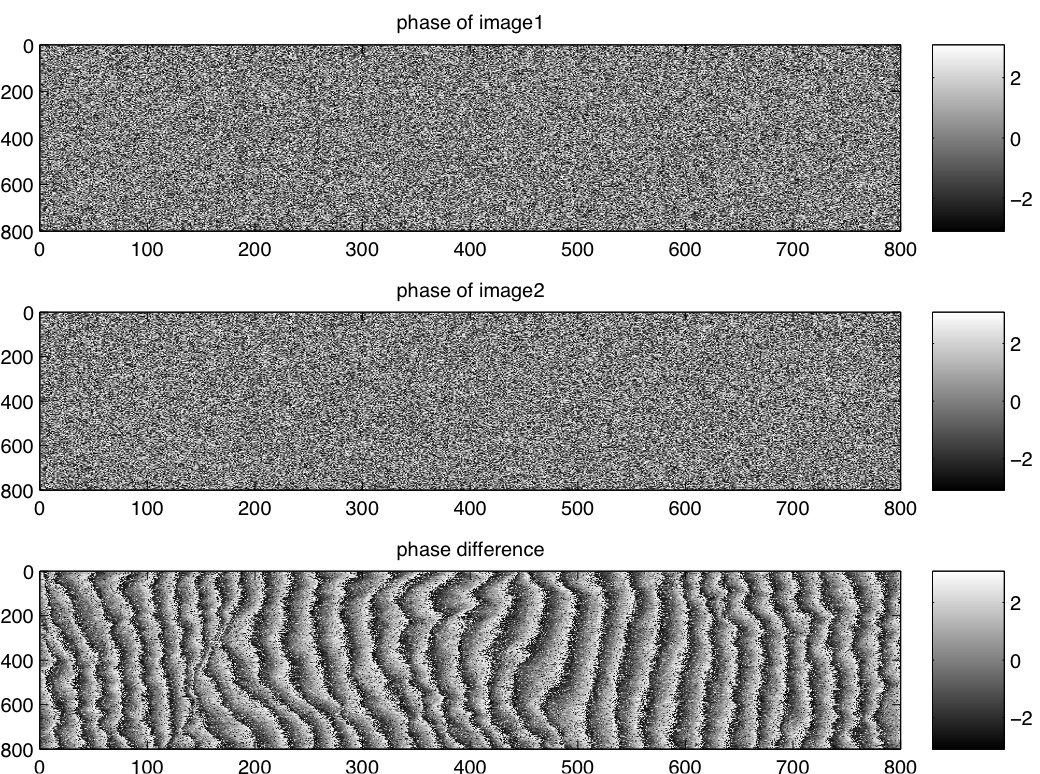
\includegraphics[width=0.7\textwidth]{insar_phase.png}
        
        \begin{align*}
            \phi\{k,l\} = & A_1\{k,l\} e^{i\psi_1\{k,l\}} \times \\
                          & A_2\{k,l\} e^{-i\psi_2\{k,l\}}
        \end{align*}
    \end{center}
\end{frame}


\begin{frame}{Phase of the interferogram}
    \[
        \subt{\Phi}{IFG} = \subt{\Phi}{defo.} + \subt{\Phi}{atmo.} + \subt{\Phi}{topo.} + \subt{\Phi}{orbit} + \subt{\Phi}{noise}
    \]
    \begin{itemize}
        \item $\subt{\Phi}{IFG}$: phase of the interferogram 
        \item $\subt{\Phi}{defo.}$ : phase caused by surface deformation, that occurred between the two SAR acquisitions, in the Line-of-Sight (LOS) direction
        \item $\subt{\Phi}{atmo.}$: phase caused by the change in atmospheric microwave propagation speed
        \item $\subt{\Phi}{topo.}$: phase due to topography
        \item $\subt{\Phi}{orbit}$: phase from errors of the orbital state vector
        \item $\subt{\Phi}{noise}$: noise from residual phase terms, that cannot be modeled
    \end{itemize}    
\end{frame}


\begin{frame}{Processing the interferometric phase}
    \[
        \subt{\Phi}{IFG} = \subt{\Phi}{defo.} + \subt{\Phi}{atmo.} + \subt{\Phi}{topo.} + \subt{\Phi}{orbit} + \subt{\Phi}{noise}
    \]
    Separation and estimation of the different phase terms:
    \begin{itemize}
        \item $\subt{\Phi}{topo.}$: using DEM, residuals correlated with baseline
        \item $\subt{\Phi}{atmo.}$: atmopsheric models, temporal filtering
        \item $\subt{\Phi}{oribt}$: more precise orbit data, deramping
        \item spatial filtering Goldstein-filter \cite{GoldsteinFilter}
    \end{itemize}
\end{frame}


\begin{frame}{Deformation}
    If estimation of $\subt{\Phi}{defo.}$ is done $\rar$ phase unwrapping $\rar$ LOS deformation.

    \begin{center}
        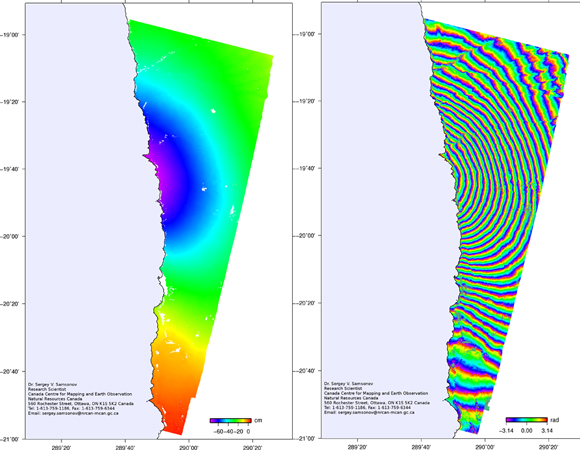
\includegraphics[width=0.55\textwidth]{wrapped_and_unwrapped_ifg.jpg}
    \end{center}

    \[
        \subt{d}{defo.} = \frac{\lambda}{4\pi} \subt{\Phi}{defo.,unwrapped}
    \]

    Multiple interferograms $\rar$ time-series analysis $\rar$ LOS deformation time-series.
\end{frame}


\def\ft{Mapping surface displacement based on natural scatterers}
\sepframe{Examples of InSAR applications: \ft}


\begin{frame}{\ft}
    \begin{itemize}
        \item $\approx$ 3.5 years of Sentinel-1 A descending orbit data (105 scenes)
        \item covering the Praid salt extrusion in Carpathian Bend area
        \item salt deformation governed by weather phenomena
        \item TopoTransyvania project: investigation of the Carpathian Bend and subduction zone
        \item analyse geodynamic processes (seismic activity, post volcanic activity, salt tectonics)
        \item SAR images processed with the Gamma Software \cite{werner2000gamma}
    \end{itemize}
\end{frame}


\begin{frame}{\ft}
    \begin{center}
        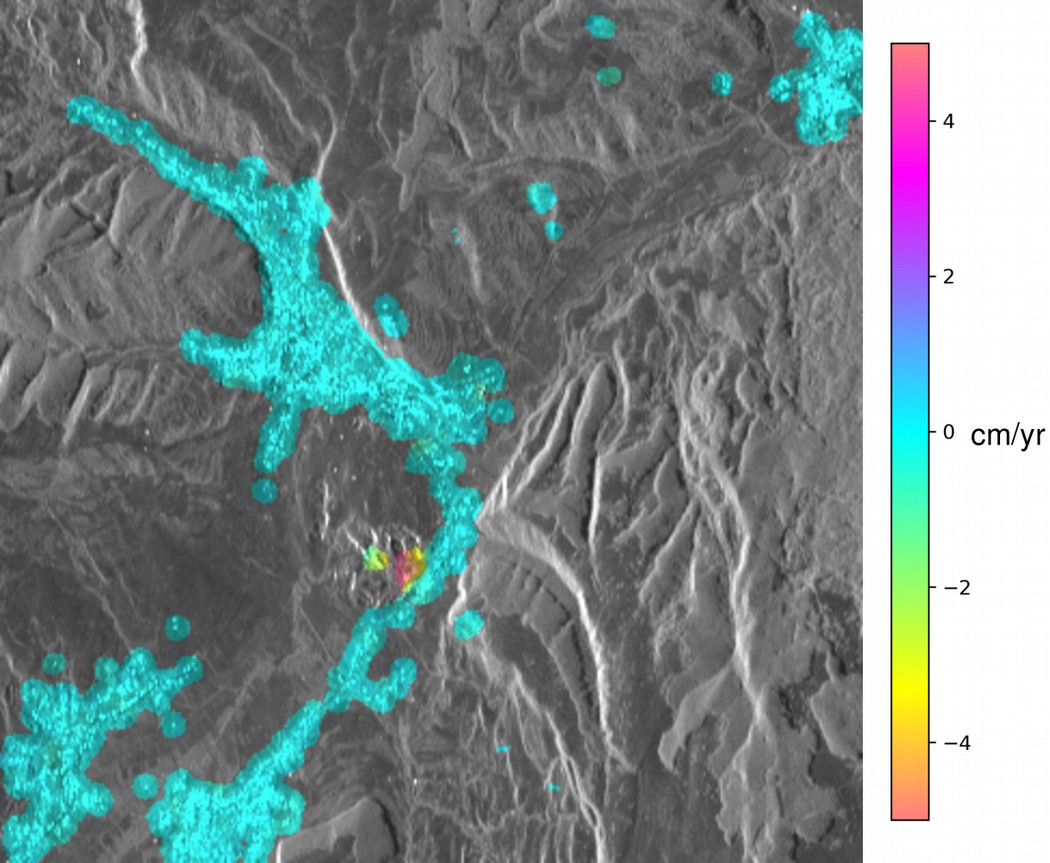
\includegraphics[width=0.6\textwidth]{parajd.png}
    \end{center}
    
    First results show deformation on the southern flanks of the salt diapir. Subsidence is in the $3-4$ cm/yr range. Lack of scatterers on the top of the salt diapir $\rar$ artificial reflectors.
\end{frame}


\begin{frame}{\ft}
    \begin{center}
        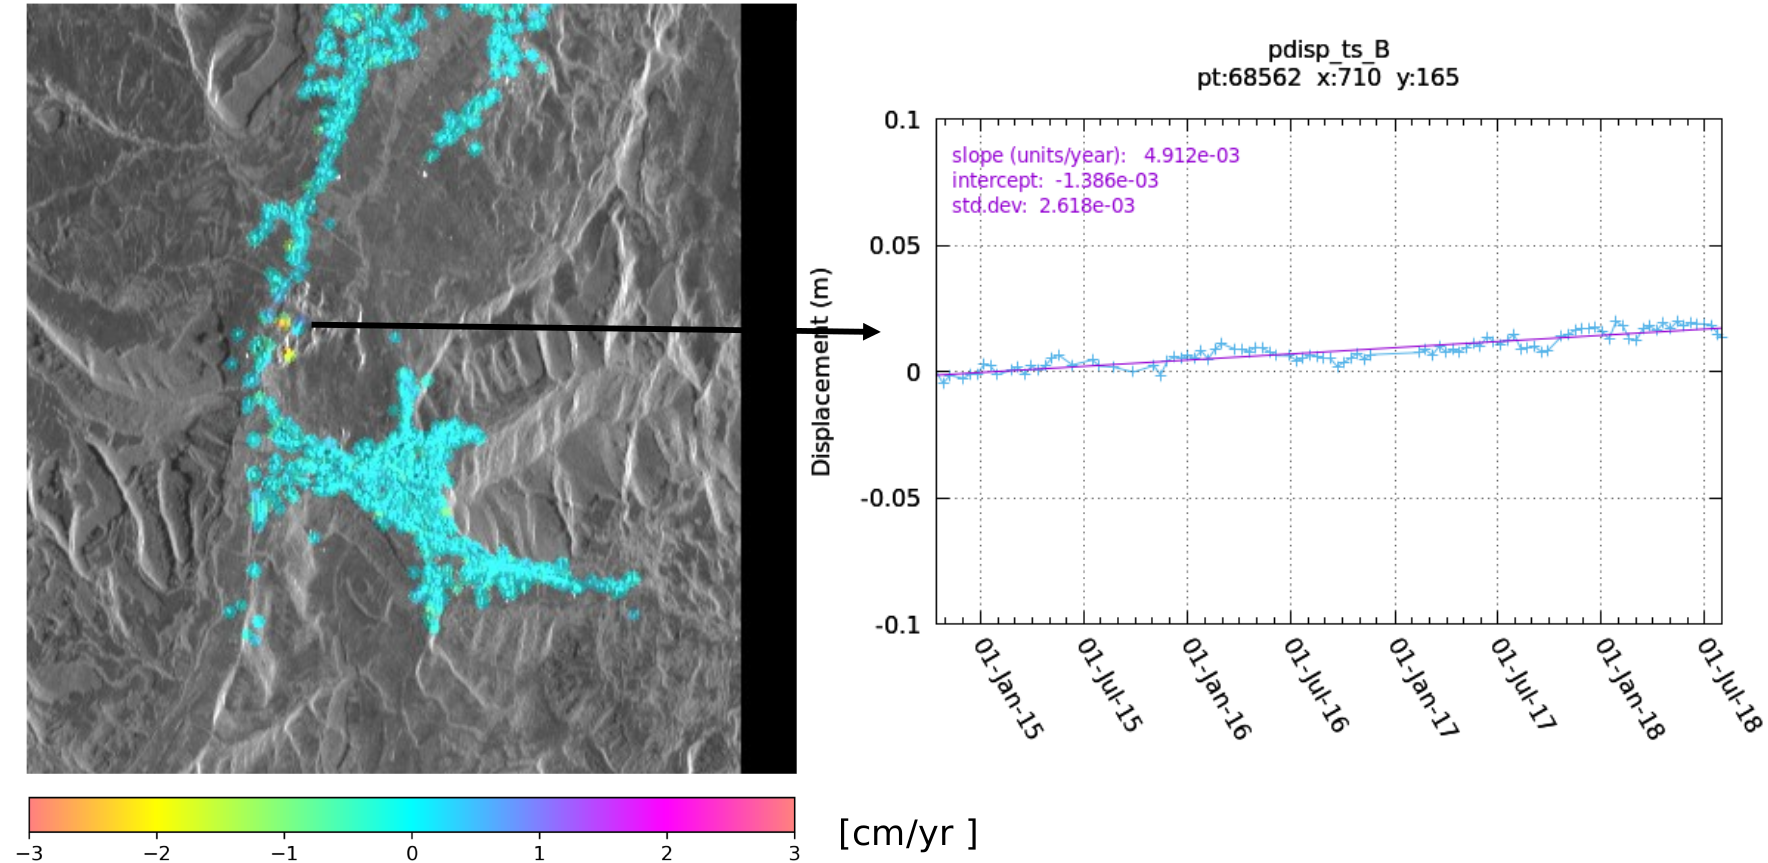
\includegraphics[width=0.8\textwidth]{parajd_ts.png}
    
    Clear trend of near constant velocity deformation away from the satellite.    
    \end{center}
\end{frame}


\def\ft{Monitoring the displacement time-series of benchmark reflector networks}
\sepframe{Examples of InSAR applications: \ft}


\begin{frame}{\ft}
    \begin{itemize}
        \item $\approx$ 1 year of Sentinel-1 A and B ascending and descending orbit data
        \item geodetic/geodynamic integrated benchmarks (IBs)
        \item IB network, settlement (Dunaszekcső) along the loess banks of the Danube
        \item GNSS measurements 1 year apart
        \item 3D displacements from combination of InSAR and GNSS data with Kalman filtering
        \item SAR images processed with Gamma and StaMPS software \cite{Hooper2008}
    \end{itemize}
\end{frame}
\begin{frame}{\ft}
    \begin{center}
        \figm{dszekcso_refl_1.jpg}{0.75}
        \vspace{10pt}
        
        Integrated benchmark on top of a subsiding loess bank of the Danube.
    \end{center}
\end{frame}


\begin{frame}{\ft}
    \begin{center}
        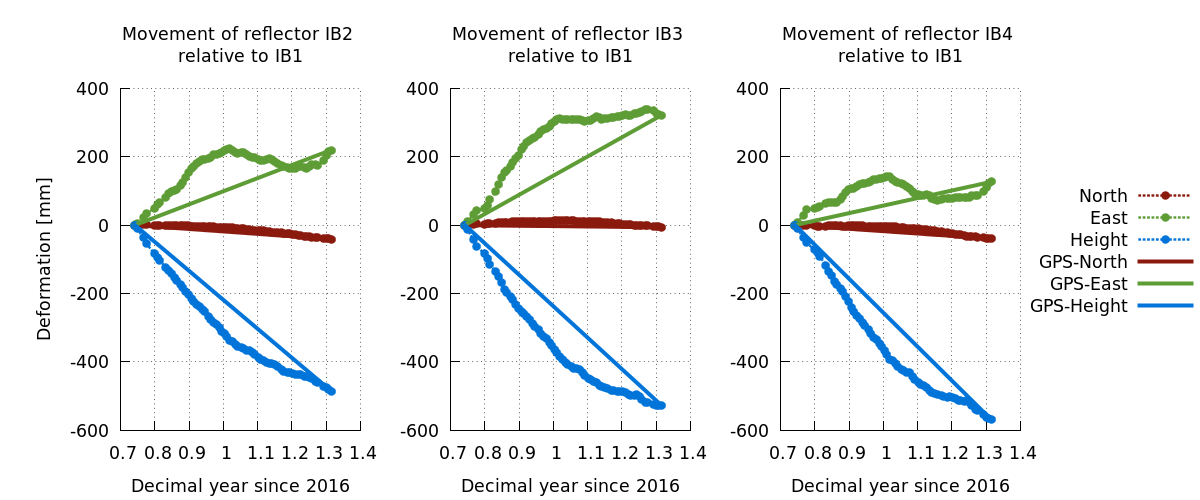
\includegraphics[width=1.0\textwidth]{dszekcso_ts.png}
        
        Similar time-series for all 3 moving reflectors, subsidence and movement towards the east (Danube).
    \end{center}
\end{frame}


\def\ft{Estimation of Integrated Water Vapor (IWV) maps using InSAR}
\sepframe{Examples of InSAR applications: \ft}


\begin{frame}{\ft}
    \begin{itemize}
        \item Sentinel-1 A and B ascending dataset covering the area around previously described benchmarks
        \item assumptions:
        \begin{itemize}
            \item no surface displacement (except for the landslide area)
            \item IFG phase due to change in IWV dominates over IFG phase caused by change in pressure and temperature profiles
        \end{itemize}
        \item estimate Zenith Wet Delay (ZWD) changes and convert into absolute ZWV using the ECMWF ERA-Interim model \cite{ERA_I}
        \item ZWD $\rar$ IWD \cite{saastamoinen1972atmospheric}:
        \begin{align*}
            \frac{\mathrm{ZWD}}{\mathrm{IWD}} &= 10^{-8} \left(k_2 - \frac{R_d}{R_w} k_1 + \frac{k_3}{T_m} \right) R_w \\
            T_m &= 70.2 + 0.72 T_s
        \end{align*}
        Constants: $k_1$, $k_2$, $k_3$, $R_d$, $R_w$ \cite{thayer1974improved, smith1953constants, hopfield1969two}
        \item SAR images processed with Gamma and StaMPS software
    \end{itemize}    
\end{frame}


\begin{frame}{\ft}
    \begin{center}
        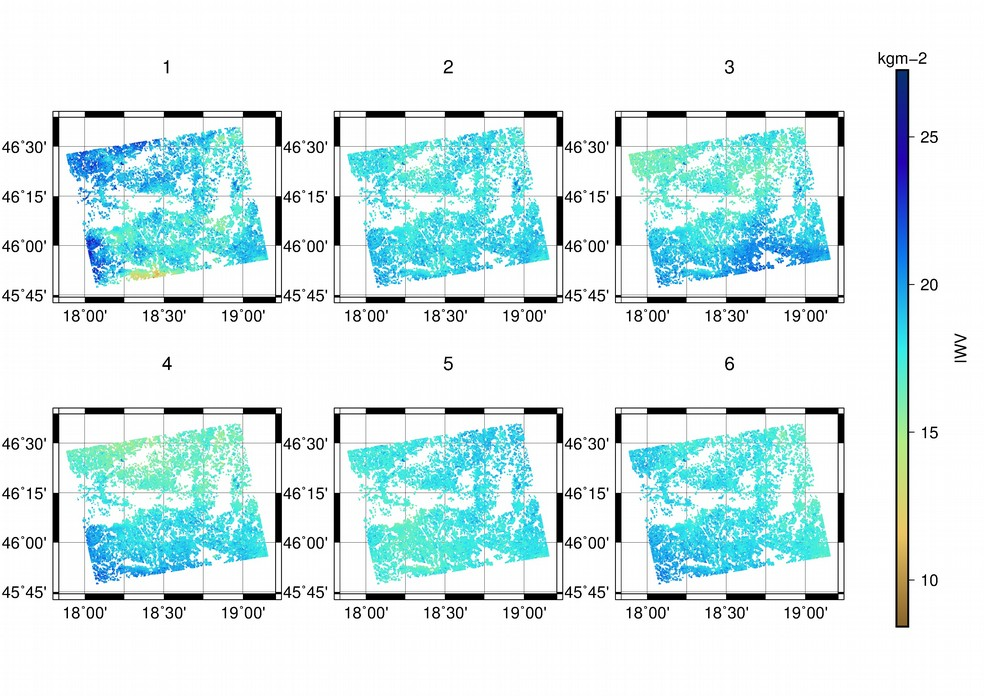
\includegraphics[width=0.85\textwidth]{iwv.png}
        \vspace{-20pt}
        
        {\small Integrated Water Vapor (IWV) values. Dates:  1 - 2016.09.24., 2 - 2016.10.06., 3 - 2016.10.16., 4 - 2016.10.24., 5 - 2016.12.30., 6 - 2016.12.05.}
    \end{center}
\end{frame}


\def\ft{Calculation of slant range ionospheric TEC differences}
\sepframe{Examples of InSAR applications: \ft}

\def\dtec{\Delta\mathrm{TEC}}

\begin{frame}{\ft}
    \begin{itemize}
        \item two PALSAR-1 SAR scenes covering the Yamagochi Prefecture in Japan, L-band, more sensitive to ionospheric effects
        \item dispersive propagation of electromagnetic waves in ionosphere, phase delay depends on frequency
        \item filtering IFG creating high and low sub-band IFGs, $\dtec$ is proportional to sub-band IFG phase differences REF
        \item robust method developed by \cite{wegmuller2018reformulating} based on \cite{meyer2006potential,gomba2015estimation}:
        \[
            \subt{\Phi}{iono.} = x \Phi_0 + y (\subt{\Phi}{high} - \subt{\Phi}{low}) = \frac{4\pi K}{c f_0} \dtec
        \]
        Constants: $x$, $y$ depend on sub-band frequencies, $K = 40.31$ $\mathrm{m}^3 \mathrm{s}^{-2}$, $c$ - speed of light, $f_0$ - radar center frequency
        \item SAR images processed with Gamma software
    \end{itemize}
    
\end{frame}


\begin{frame}{\ft}
    \begin{minipage}[c]{0.7\textwidth}
        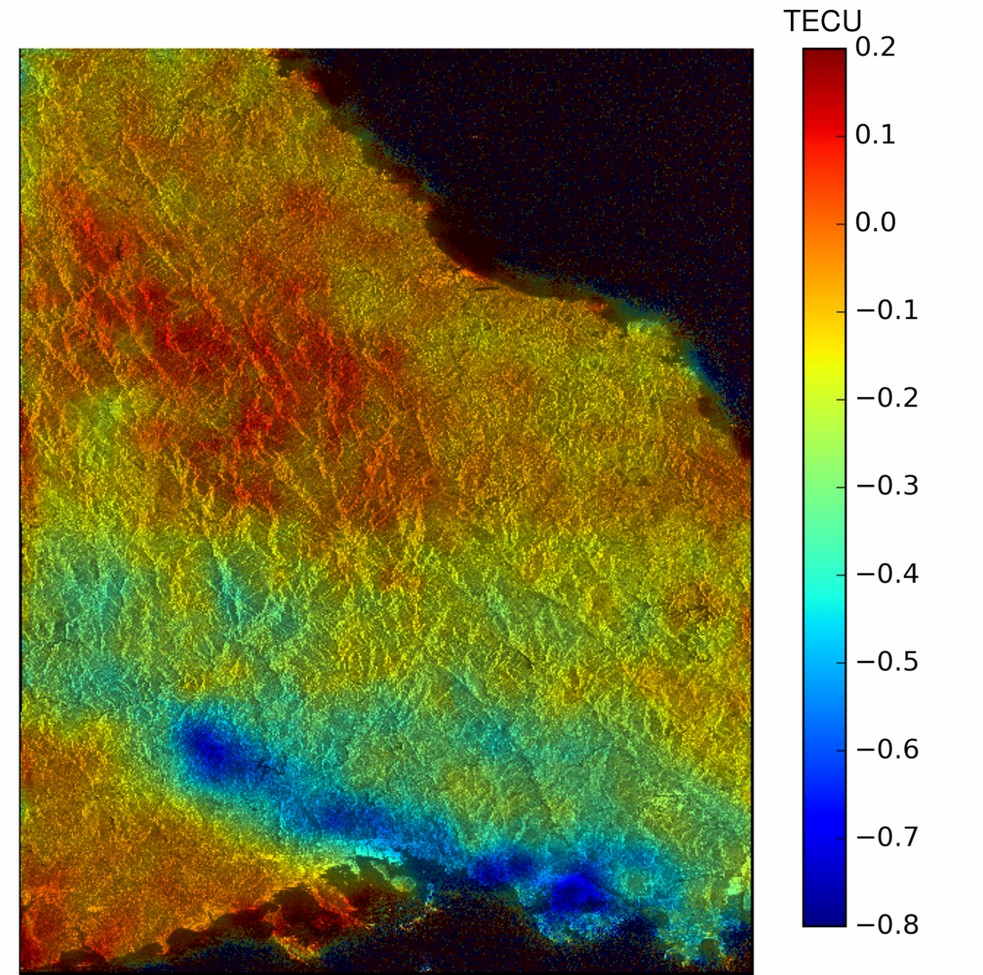
\includegraphics[width=1.0\textwidth]{iono.png}
    \end{minipage}
    \begin{minipage}[c]{0.28\textwidth}
         Total Electron Content (TEC) changes between 2009.03.28. and 2009.06.28. above the Yamagochi Prefecture Japan. TEC changes are relative to the upper left corner of the SAR scene. 1 TECU = $10^{16}$ $\mathrm{electron} / \mathrm{m}^2$. Background image is the SAR backscatter intensity image of the 2009.03.28. scene.
    \end{minipage}
\end{frame}


\begin{frame}{}

    {\Large \fcol Discussion}
    
    \begin{itemize}
        \item multiple applications of InSAR technology
        \item Sentinel-1 extremely useful for monitoring surface deformation
        \item estimation of slant-range and vertical integrated quantities (IWV, TEC) describing the state of the atmosphere
        \item long-term time series of integrated quantities: trends, their correlation, troposphere - ionosphere interaction
    \end{itemize}
    
    \vspace{10pt}
    
    {\Large \fcol Future plans}
    
    \begin{itemize}
        \item Refinement of deformation monitoring techniques.
        \item Validation of derived IWV and $\dtec$ values using independent data sources (weather models, ionosonde data).
        \item $\dtec$ estimation based on Sentinel-1 images
        \item IWV calculation without the need for auxiliary data (weather model).
    \end{itemize}
\end{frame}


\begin{frame}
    \begin{center}
        \Huge \fcol
        Thank you for your attention!
    \end{center}
    \vspace{25pt}
    
    \begin{center}
        \Large \fcol \center Acknowledgement
    \end{center}
    \vspace{10pt}
    
    Contains modified Copernicus Sentinel data 2014-2018, processed by ESA.
    \vspace{5pt}
    
    This study was supported by the TopoTransylvania - a multidisciplinary Earth science initiative in Central Europe to tackle local and global challenges project (NKFI NN 128629).
\end{frame}


\begin{frame}[allowframebreaks]{Bibliography}
    \tiny\bibliography{../../../insar}
    \bibliographystyle{apalike}
\end{frame}

\end{document}
